\chapter{Lightweight Scene Understanding}

\section{Task Definition}
%The first part of the proposed framework deals with obtaining accurate semantic labeling from images captured by the navigation camera on Mars Rover. This is an essential step to aid the rover in achieving autonomous navigation, considering the delay in communications between Mars and Earth and real-time ground control is not practicable.
%In this section a deep-learning approach was implemented to tackle this task, given the vast progress made in semantic segmentation techniques in the field. The main objective was to test several Deep Learning architectures on a novel benchmark dataset [Mars Bench with S5Mars] that provided accurate labels for both terrain segmentation but that could also be useful for the second part in identifying rover parts in the image. Importance was also given to the efficiency of techniques used, looking for a possible on-board deployment that requires a lot of constraint to be effectively operatable, such as ...
%so accuracy-efficiency tradeoff was an important factor used when choosing and optmizing the architectures.

The one-way light time between Earth and Mars varies from approximately 4 to 22 minutes, making continuous remote operations impracticable \cite{nasaJPL2022Driving}. Decisions that must be taken while a rover traverses terrain not yet examined by ground operators therefore benefit from onboard perception and autonomous reasoning. The first branch of the proposed framework addresses this perception problem through semantic segmentation of rover-acquired RGB imagery. More specifically, the experiments presented in this thesis use images captured by the Mast Camera (Mastcam) aboard the Curiosity rover, as provided by the Mars-Bench release of S5Mars \cite{zhang2024s5mars,purohit2025marsbench}. The objective is to convert each observation into a pixel-level representation of the surrounding scene that may support downstream functions such as terrain interpretation, traversability assessment, and route planning.
The dataset was selected because its label space covers terrain elements relevant to environmental understanding while also including a \emph{Rover} category, establishing a possible future interface with the damage-inspection branch.

A deep learning approach is adopted to compare architectures with different representational capacities and computational requirements. The objective is not to maximize segmentation accuracy in isolation, because potential onboard use makes computational efficiency a central design criterion, as also emphasized by previous research on lightweight semantic segmentation for Martian environments \cite{xiong2024light4mars}. The experimental study therefore considers the accuracy-efficiency trade-off and subsequently investigates quantization as a means of reducing inference cost without introducing an unacceptable degradation in segmentation quality.

\section{Dataset}
The primary dataset adopted for the scene-understanding experiments is the Mars-Bench adaptation of S\textsuperscript{5}Mars. The original S\textsuperscript{5}Mars dataset was introduced by Zhang et al. for semi-supervised semantic segmentation of Martian scenes \cite{zhang2024s5mars}. It comprises 6,000 RGB images acquired by the Mast Camera (Mastcam) aboard the Curiosity rover, each with a spatial resolution of 1200 $\times$ 1200 pixels. Its annotations follow a sparse, confidence-based protocol, where instead of assigning a category to every pixel, labels are retained only in regions for which the annotators considered the semantic interpretation sufficiently reliable. This design limits uncertain assignments at visually ambiguous boundaries, but also leaves part of each mask without a terrain label.

The Mars-Bench release was selected in preference to the original distribution to obtain a more reproducible and internally consistent evaluation protocol. Mars-Bench converts previously published Martian vision datasets into standardized formats and supplies predefined training, validation, and test partitions \cite{purohit2025marsbench}. More importantly, its authors subjected the terrain-segmentation datasets to an additional expert review. They reported ambiguities among visually similar granular-material categories and consolidated the corresponding S\textsuperscript{5}Mars labels into a single \emph{Sand/Soil} category. This refinement was intended to reduce label noise and make comparisons between models less dependent on uncertain distinctions. This Mars-Bench release used in this work contains 4,997 training images, 200 validation images, and 800 test images. Mars-Bench describes eight target categories, while the released masks expose an additional \emph{Background} identifier. Consequently, the implementation uses nine mask identifiers: \emph{Background}, \emph{Bedrock}, \emph{Hole}, \emph{Ridge}, \emph{Rock}, \emph{Rover}, \emph{Sand/Soil}, \emph{Sky}, and \emph{Track}

Two additional datasets included in Mars-Bench were used for a separate cross-dataset evaluation: MarsSeg MSL and MarsSeg MER \cite{purohit2025marsbench}. Both originate from the Mars-Seg dataset family introduced by Li et al. \cite{li2022covda} and were subsequently adapted to the standardized taxonomy and evaluation protocol defined by Mars-Bench. MarsSeg MSL comprises RGB Mastcam images acquired by the Curiosity rover during the Mars Science Laboratory (MSL) mission, whereas MarsSeg MER contains grayscale images captured by the Navigation Cameras (Navcams) and Panoramic Cameras (Pancams) aboard the Spirit and Opportunity rovers during the Mars Exploration Rover (MER) missions \cite{li2022covda}. Their identical label mapping permits direct cross-mission evaluation without modifying the output layer or introducing an uncertain correspondence between categories. A model can be trained and selected using one mission and subsequently evaluated, without target-domain fine-tuning, on the test split of the other.

\begin{table}[ht]
\centering
\resizebox{\linewidth}{!}{%
\begin{tabular}{@{}l l c r r r@{}}
\toprule
\textbf{Dataset} &
\textbf{Rover(s) / Sensor(s)} &
\textbf{Mask IDs} &
\textbf{Training} &
\textbf{Validation} &
\textbf{Test} \\
\midrule
\midrule
S\textsuperscript{5}Mars
& Curiosity / Mastcam
& 9 & 4,997 & 200 & 800 \\
MarsSeg MSL
& Curiosity / Mastcam
& 7 & 2,893 & 413 & 828 \\
MarsSeg MER
& Spirit, Opportunity / Navcam, Pancam
& 7 & 744 & 106 & 214 \\
\bottomrule
\end{tabular}%
}
\vspace{5mm}
\caption{Mars-Bench semantic segmentation datasets used in this work. The number of mask identifiers includes the \emph{Background} label.}
\label{tab:mars-bench-datasets}
\end{table}

\section{Pre-processing}

A consistent input representation was enforced across all dataset splits. Each image was converted to RGB, ensuring a three-channel input irrespective of its original encoding, while the corresponding segmentation mask was retained as a single-channel categorical map. Image-mask pairs were subsequently resized to \(512 \times 512\) pixels, a resolution selected to retain sufficient spatial detail for semantic segmentation. Bilinear interpolation was used for the RGB images, as it provides smooth resampling of continuous intensity values, while nearest-neighbour interpolation was applied to the segmentation masks to prevent the introduction of intermediate values that would not correspond to valid semantic categories.

Data augmentation was implemented as an optional training-only stage after resizing. The available transformations comprised horizontal flipping, vertical flipping and random \(90^{\circ}\) degree rotations with probability \(0.5\). When the rotation operation was triggered, the number of \(90^{\circ}\) rotations was sampled uniformly from \(k \in \{0,1,2,3\}\). The default configuration disabled augmentation, whereas the augmented configurations activated these transformations explicitly for comparative experiments. Following the optional augmentation stage, images were scaled to the \([0,1]\) range and then channel-wise normalization was performed using the ImageNet mean values and standard deviations. This convention maintains compatibility with the ImageNet-pretrained encoders employed by several of the evaluated architectures. Segmentation masks were instead converted to integer tensors without normalization, thereby preserving their original class identifiers.
No stochastic transformation was applied to the validation or test sets, as their samples underwent only the deterministic operations of RGB conversion, resizing, tensor conversion, and normalization, ensuring that the reported evaluation results were not affected by random data transformations.

\section{Segmentation Architectures}
\label{sec:segmentation-architectures}

The architecture set was selected with two complementary objectives: preserving continuity with the segmentation models considered in Mars-Bench and investigating a sufficiently broad accuracy-efficiency spectrum for potential onboard deployment. Mars-Bench includes U-Net, DeepLabV3+, SegFormer, and DPT among its semantic segmentation baselines \cite{purohit2025marsbench}. Three of these, U-Net, DeepLabV3+, and SegFormer, were retained in this work. DeepLabV3 was added to examine an atrous-convolution architecture without the low-level feature decoder introduced in DeepLabV3+, whereas LCNet$_{3,7}$ and LCNet$_{3,11}$ were included as explicitly novel lightweight alternatives.

The resulting model pool comprises seven configurations and covers four substantially different design principles: skip-connected convolutional encoder-decoders, atrous spatial pyramid pooling, hierarchical Transformer representations, and partial-channel transformations. This diversity makes it possible to investigate whether the gains associated with increasingly expressive context modeling justify their computational cost. % At the same time, the experiments presented in this thesis should not be interpreted as a strict reproduction of the Mars-Bench baseline study. The selected backbones, initialization schemes, optimization procedure, and evaluation protocol are specific to the present work; the relationship with Mars-Bench is therefore one of architectural continuity rather than direct leaderboard comparability.

For the S5Mars experiments, every architecture received a three-channel image resized to \(512 \times 512\) pixels and produced nine channels of raw logits at the same spatial resolution, one for each class in the taxonomy. No activation function was incorporated into the final segmentation head, allowing the training objective to operate directly on the logits. All network components were left trainable.

The U-Net and DeepLab configurations were instantiated through the Segmentation Models PyTorch library \cite{iakubovskii2019smp}. Their encoders were initialized using weights learned on ImageNet, while their decoders and segmentation heads were initialized for the target task. SegFormer-B0 was instead initialized from a checkpoint fine-tuned for semantic segmentation on ADE20K \cite{nvidiaSegformerB0}, with its incompatible 150-class classifier replaced by a nine-channel layer, while the compatible encoder and decoding weights were retained. The two LCNet configurations were trained from random initialization, given the absence of pretrained weights. Consequently, comparisons among different model families capture the behavior of complete deployment candidates, including their initialization strategy, and should not be interpreted as controlled ablations of architecture alone.

\subsection{U-Net Variants}

% U-Net is a Convolutional Neural Network (CNN) Architecture, that follows a symmetric encoder-decoder organization originally introduced for biomedical image segmentation \cite{ronneberger2015unet}. Its contracting path progressively reduces the spatial resolution of the input while extracting increasingly abstract representations, allowing the network to incorporate a broader image context. The expanding path reverses this process and reconstructs a dense prediction at progressively finer resolutions. The defining feature of the architecture is the set of skip connections between corresponding encoder and decoder stages. These connections transfer higher-resolution features directly to the decoding path, where they are combined with more contextual but spatially coarser representations. The decoder can therefore recover local information that would otherwise be weakened by repeated downsampling. This property makes U-Net a suitable conventional and efficient baseline for terrain segmentation, where the accurate localization of class boundaries is important.

The U-Net is a Convolutional Neural Network (CNN) Architecture, which consists
of symmetric encoder-decoder architecture that was originally proposed for biomedical image segmentation tasks \cite{ronneberger2015unet}. The contracting path reduces the spatial resolution of the input and extracts abstract representation of the data, thus enabling the network to encode a wider context of the image. The expansion path is the opposite, it restores a dense output representation at progressively higher resolutions. The defining characteristic of this architecture is skip connections between pairs of corresponding encoder-decoder stages. Skip connections pass higher resolution features directly to the decoder, where they can be combined with features having more context but lower resolution. Thus, the decoder is able to restore local information, which can be lost during multiple downsamplings. This allows using the U-Net as an appropriate baseline for terrain segmentation task due to the importance of class boundaries location. 

\begin{figure}[ht!]
\centering
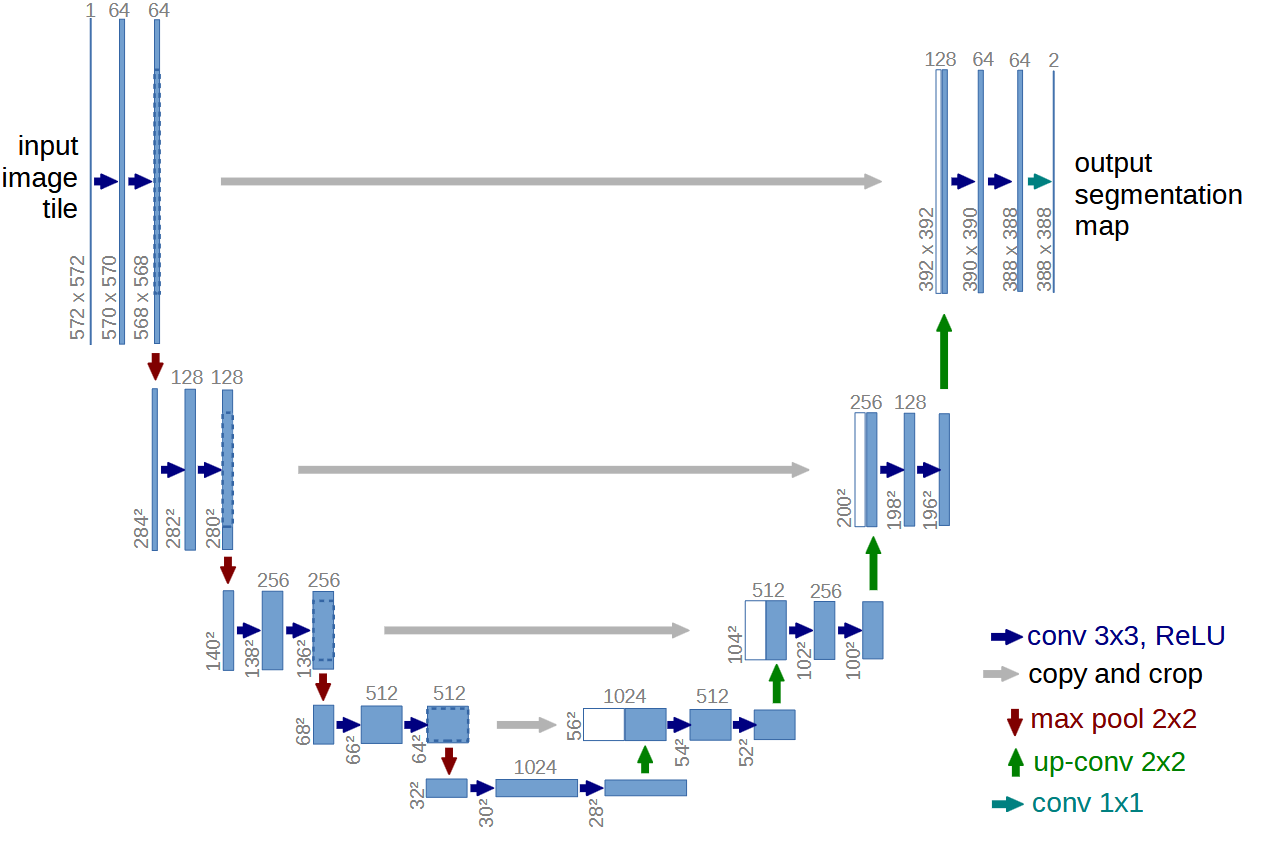
\includegraphics[width=0.95\textwidth]{Images/original-unet.png}
\vspace{3mm}
\caption{The original U-Net architecture proposed by Ronneberger et al., comprising a contracting path, an expanding path, and skip connections between corresponding resolution levels \cite{ronneberger2015unet}. The implementations evaluated in this work replace the original contracting path with ResNet-34 or MobileNetV2.}
\label{fig:unet}
\end{figure}

% Both U-Net configurations employed a five-stage decoder, where at each stage the decoder representation was upsampled using nearest-neighbor interpolation, concatenated with the corresponding encoder feature map, and processed by two convolutional blocks with batch normalization and ReLU activation.
Both U-Net variants had a five-stage decoder where, at each stage, the decoder representation was upscaled using nearest-neighbor interpolation and concatenated with the corresponding encoder representation followed by two \(3 \times 3\) convolutional blocks with batch normalization and ReLU activation. A final \(3 \times 3\) segmentation head mapped the resulting 16-channel representation to the nine output classes.

\paragraph{U-Net with ResNet-34.}

The first variant makes use of ResNet-34 as the encoder. ResNets are a type of architecture that stacks the convolutional layers in blocks where the learned transformation of the block is added to the original block input via a shortcut connection \cite{he2016resnet}. Therefore, every block learns to correct the original representation rather than learning a completely new transformation. ResNet was proposed by He et al. as a way of solving the optimization degradation problem that is experienced when increasing the depth of the conventional convolutional networks. When the input and output dimensions agree, the identity shortcut introduces neither additional parameters nor a separate learned transformation.

In the case of U-Net, ResNet-34 provides a conventional hierarchical encoder whose intermediate representations can be transferred to the decoder at different spatial scales. The choice of this architecture was motivated by the fact that it was a higher-capacity convolutional variation in the U-Net family. It combines the established residual feature extractor with an explicit reconstruction path for dense prediction, while preserving architectural continuity with the U-Net baseline considered in Mars-Bench.

The same ResNet-34 encoder is also employed in the DeepLabV3 configuration described later in this section. Although the resulting networks are not identical outside the encoder, this shared component makes the comparison between skip-based reconstruction and ASPP-based context aggregation easier to interpret.

\paragraph{U-Net with MobileNetV2.}

The second variant replaces ResNet-34 with MobileNetV2, an architecture developed specifically for mobile and resource-constrained computer vision \cite{sandler2018mobilenetv2}. MobileNetV2 is an improved version of MobileNetV1, with the aim of optimizing accuracy while ensuring efficiency \cite{lightweight-survey}. Its central component is the inverted residual block.  Whereas the traditional residual block transforms the input representation in the middle of relatively wider representations, MobileNetV2 does this task in between narrower representations, known as bottlenecks. Each block first expands the input representation, performs spatial filtering through an inexpensive depthwise convolution, and then projects the result back to a lower-dimensional space. The final projection is linear, since Sandler et al. observed that applying a non-linearity within a narrow bottleneck can lose useful representational information.

Inside each inverted residual block, depthwise convolution applies a spatial filter independently to every expanded feature channel, whereas the preceding and subsequent pointwise convolutions expand, combine, and project the channel representations. By using spatial filtering and channel mixing in this manner, MobileNetV2 reduces the computational cost associated with typical dense convolutions, while residual connections preserve information between bottleneck representations whenever their spatial resolution and channel dimensionality remain unchanged \cite{sandler2018mobilenetv2}.

The variant was therefore included to determine whether the U-Net topology could provide an effective segmentation model with a substantially lighter encoder. Its comparison with the ResNet-34 variant examines two deployment alternatives using the same architectural family: one centered on a conventional residual hierarchy and the other on mobile-oriented inverted residual blocks.

\begin{figure}[ht!]
\centering
\begin{subfigure}[t]{0.38\textwidth}
\centering
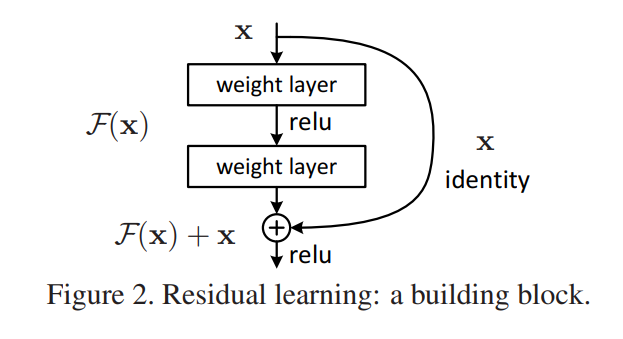
\includegraphics[width=\linewidth]{Images/Residual Connection.png}
\caption{Residual learning block.}
\label{fig}
\end{subfigure}
\hfill
\begin{subfigure}[t]{0.56\textwidth}
\centering
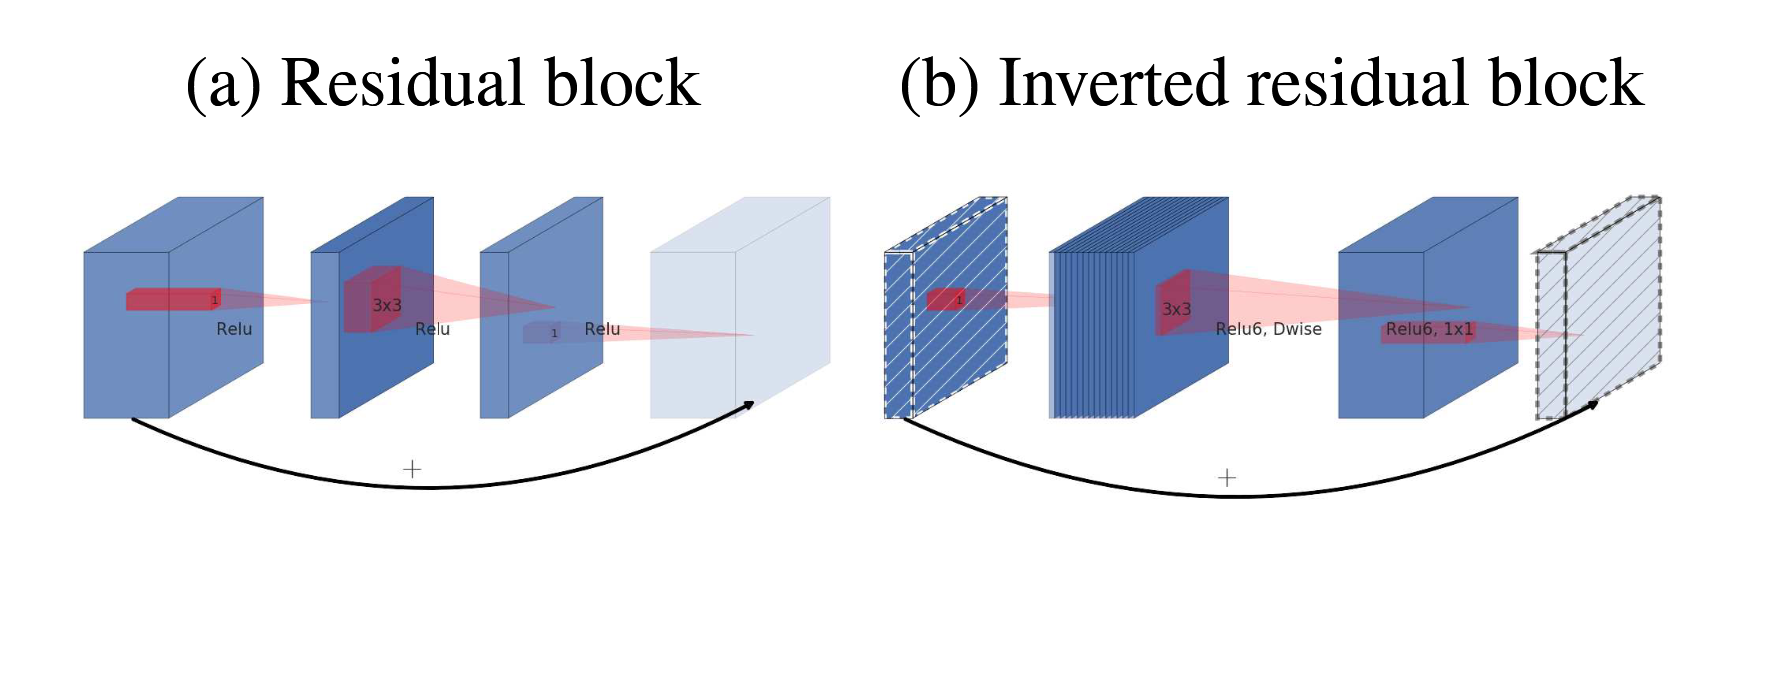
\includegraphics[width=\linewidth]{Images/Mobilenetv2.png}
\caption{Conventional and inverted residual blocks.}
\label{fig}
\end{subfigure}
\vspace{3mm}
\caption{Original diagrams illustrating the principles underlying the two U-Net encoders. The residual learning block in (a) is reproduced from He et al. \cite{he2016resnet}; the comparison between conventional and inverted residual blocks in (b) is reproduced from Sandler et al. \cite{sandler2018mobilenetv2}. Block width in the MobileNetV2 diagram represents the relative number of channels.}
\label{fig:resnet-mobilenet}
\end{figure}

\subsection{DeepLab Variants}

Semantic segmentation requires a model to preserve sufficiently detailed spatial information while also capturing the larger context needed to classify each image region. Conventional classification backbones gradually reduce feature-map resolution through strided convolutions and pooling, in a way that can discard spatial information that remains relevant to dense prediction. The DeepLab family addresses this aspect primarily through atrous convolution, also known as dilated convolution \cite{chen2017deeplabv3}.

Atrous convolution introduces spacing between the positions sampled by a convolutional filter. Increasing this spacing enlarges the effective field of view without increasing the number of learned kernel parameters and it can produce denser final feature maps while retaining a broad receptive field \cite{chen2017deeplabv3}. The atrous rate determines the spacing, with a rate of one corresponding to conventional convolution. DeepLabV3 applies this operation within an Atrous Spatial Pyramid Pooling (ASPP) module. ASPP sends the encoder output through several parallel branches whose different atrous rates capture context over different spatial extents. A separate image-pooling branch summarizes the complete feature map and supplies global contextual information. The outputs are then merged to form the representation used for pixel classification \cite{chen2017deeplabv3}.

This multi-scale mechanism is relevant to Martian scene understanding,
where terrain features exhibit substantial variations in spatial scale.
Previous work has addressed this challenge by combining multi-scale
feature extraction with the preservation of local details and small
objects \cite{li2025marsseg}. These considerations motivate the use of
both broad contextual information and localized evidence in the present
work.

\begin{figure}[ht!]
\centering
\begin{subfigure}[t]{0.43\textwidth}
\centering
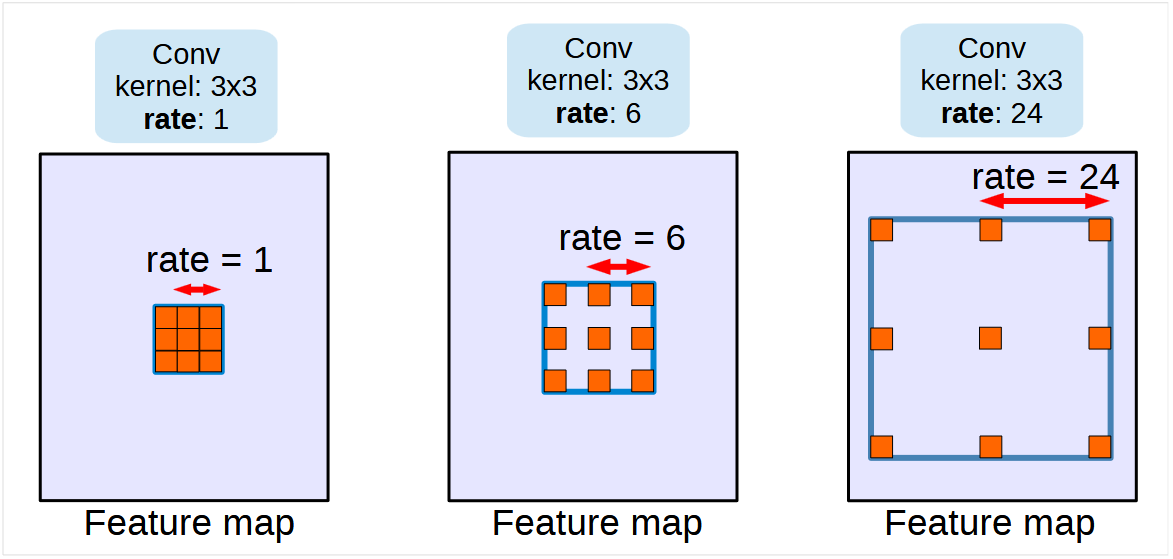
\includegraphics[width=\linewidth]{Images/deeplabv3_original_figure1.png}
\caption{Atrous convolution at different sampling rates.}
\label{fig}
\end{subfigure}
\hfill
\begin{subfigure}[t]{0.53\textwidth}
\centering
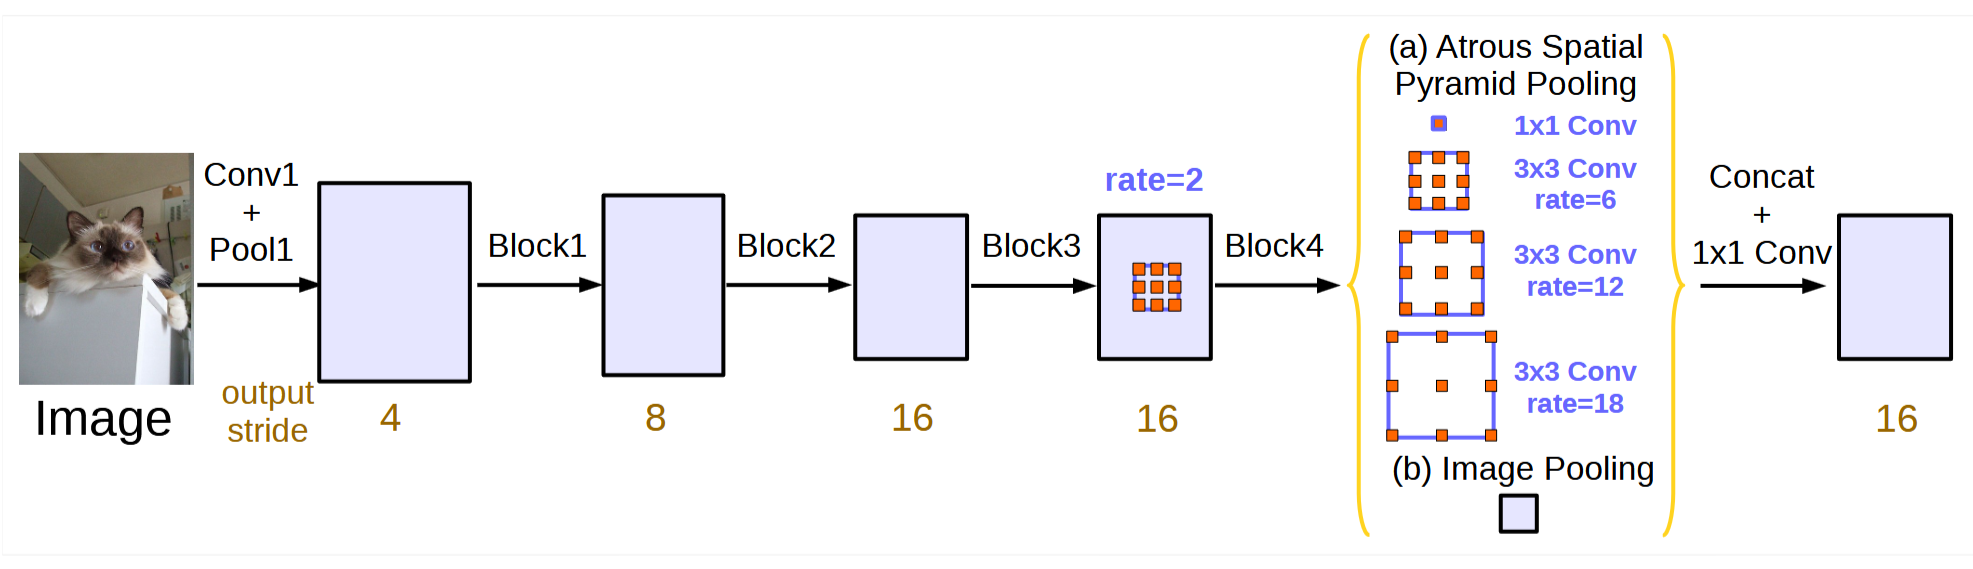
\includegraphics[width=\linewidth]{Images/deeplabv3_original_figure5.png}
\caption{ASPP augmented with image-level features.}
\label{fig}
\end{subfigure}
\vspace{3mm}
\caption{Original diagrams illustrating the principal operations of DeepLabV3. Atrous convolution enlarges the effective field of view by changing the sampling rate, while ASPP combines parallel context branches and image-level pooling. Both diagrams are taken from Chen et al. \cite{chen2017deeplabv3}.}
\label{fig}
\end{figure}

\paragraph{DeepLabV3 with ResNet-34.}

The first variant uses ResNet-34 as its encoder. Unlike U-Net, DeepLabV3 does not use a multi-stage decoder with skip connections. Instead, the ASPP features are converted into class logits and resized to the input resolution using bilinear interpolation \cite{chen2017deeplabv3}.
This variant was selected to compare two segmentation approaches built around the same backbone. U-Net--ResNet-34 progressively combines encoder and decoder features to recover spatial detail, whereas DeepLabV3 gathers multi-scale context at the final encoder stage. Other architectural differences mean that this comparison does not isolate the decoder alone, but it helps examine the strengths of each approach. DeepLabV3 also provides a reference for discussing DeepLabV3+, whose additional decoder uses low-level features to refine the segmentation boundaries.

\paragraph{DeepLabV3+ with MobileNetV2.}

DeepLabV3+ extends the predecessor by combining its multi-scale contextual encoder with a lightweight decoder \cite{chen2018deeplabv3plus}. The ASPP representation is first upsampled and then merged with an earlier feature map from the backbone, providing information that can support the refinement of object and region boundaries. The fused features are processed by the decoder before a final upsampling operation restores the prediction to the input resolution.

The resulting architecture combines two complementary mechanisms. Atrous convolution and ASPP encode contextual information over several spatial ranges, while the decoder reintroduces higher-resolution information that is less accessible from the deepest feature map alone. The original DeepLabV3+ study further employed depthwise-separable convolutions within the ASPP and decoder modules to reduce their computational cost \cite{chen2018deeplabv3plus}.

\begin{figure}[ht!]
\centering
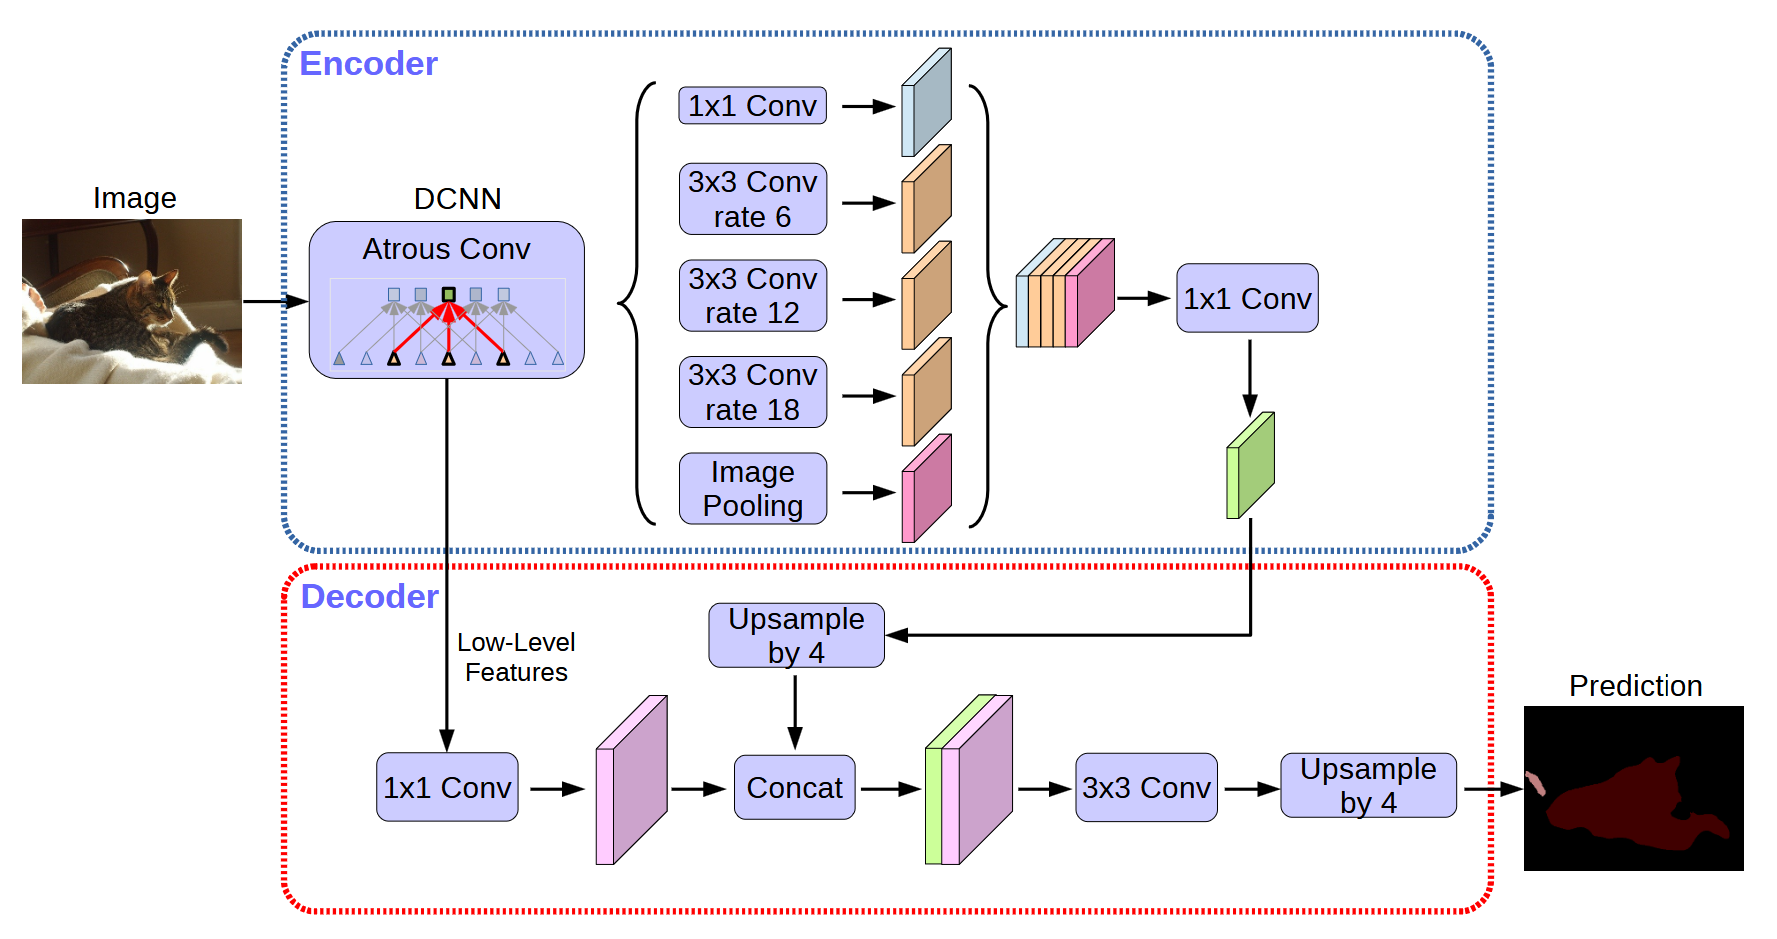
\includegraphics[width=0.9\textwidth]{Images/deeplabv3plus_original_figure2.png}
\vspace{3mm}
\caption{Original DeepLabV3+ architecture, Reproduced from Chen et al. \cite{chen2018deeplabv3plus}.}
\label{fig}
\end{figure}

The second variant makes use of the same MobileNetV2 backbone utilized by the previous U-Net configuration, providing a second cross-family point of comparison. This choice produces a deployment-oriented configuation of DeepLabV3+ rather than reproducing the modified Xception backbone emphasized in the original paper.

\subsection{SegFormer-B0}

SegFormer combines a hierarchical Transformer encoder, called Mix Transformer (MiT), with a lightweight multilayer perceptron (MLP) decoder \cite{xie2021segformer}. The architecture was included to examine attention-based alternative to the convolutional models described above.

Self-attention allows each position to gather information from distant parts of the image within a single layer, whereas local convolutions build larger context through successive layers \cite{vaswani2017attention}. For Martian semantic segmentation, this provides a reason to investigate whether relationships across an image can help discriminate terrain regions whose local appearance may be ambiguous.
MiT extracts features in four stages, producing progressively larger representations. Overlapping patch embeddings preserve local continuity, while attention uses spatially reduced features to lower its computational cost. Each block also includes a Mix-FFN module, which adds local spatial information through a depthwise convolution. This removes the need for explicit positional embeddings and their interpolation when the input resolution changes \cite{xie2021segformer}.

The decoder projects the four encoder outputs into a common feature dimension, resizes them to the same spatial resolution, and fuses them before classification \cite{xie2021segformer}. This brings all encoder stages together in a single fusion step, therefore its evaluation examines whether this compact decoder can preserve the spatial detail needed for terrain segmentation.

\begin{figure}[ht!]
\centering
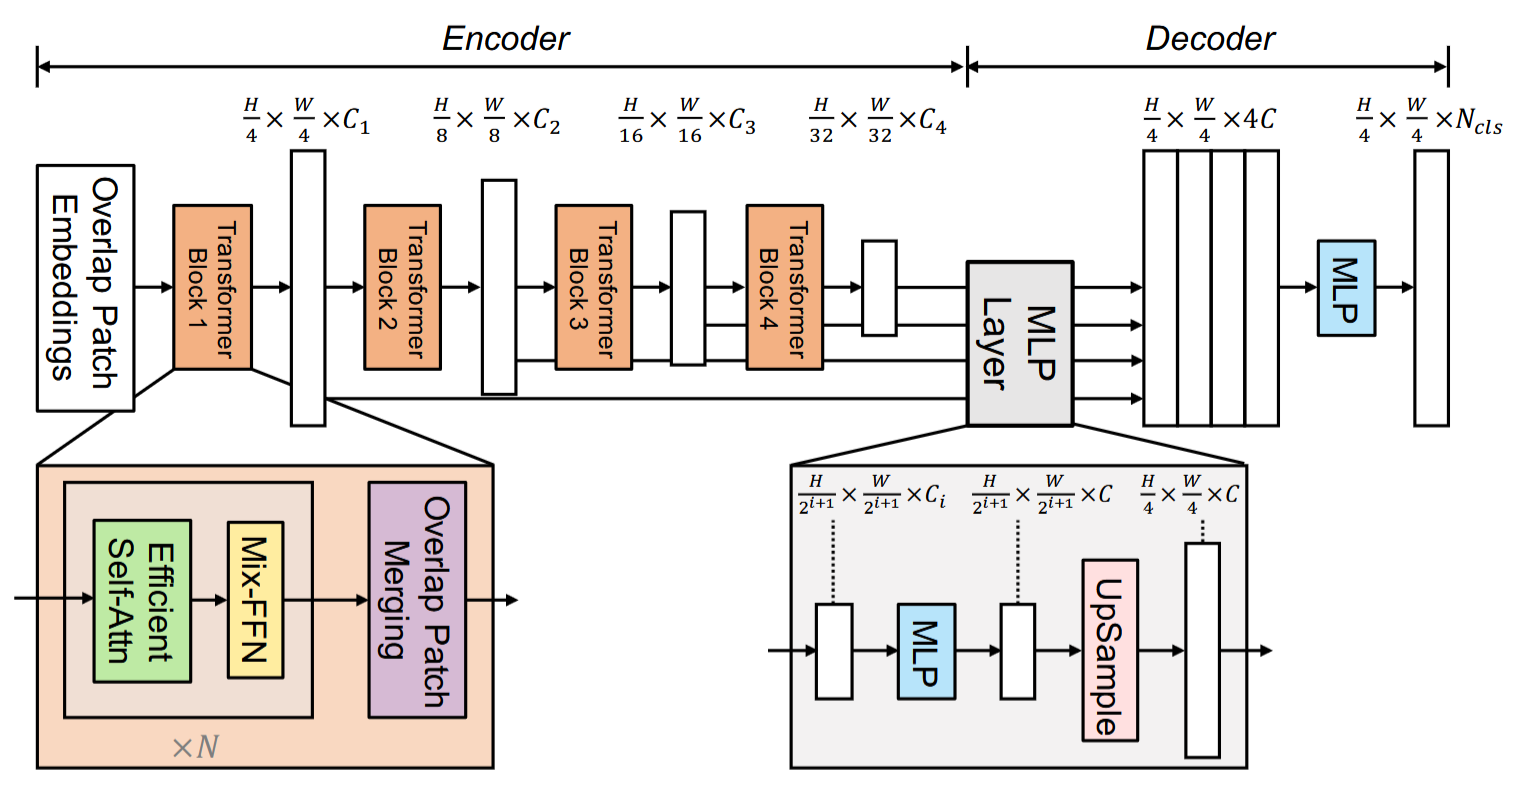
\includegraphics[width=\textwidth]{Images/segformer_original_figure2.png}
\vspace{3mm}
\caption{Original SegFormer architecture, showing the hierarchical Transformer encoder and the decoder that fuses its outputs. Reproduced from Xie et al. \cite{xie2021segformer}.}
\label{fig}
\end{figure}

SegFormer was included because it is one of the model families evaluated in Mars-Bench \cite{purohit2025marsbench}. B0, its smallest variant, was selected to limit model size \cite{xie2021segformer}, while testing its accuracy-efficiency trade-off, with results presented in the evaluation chapter. The model was initialized from \texttt{nvidia/segformer-b0-finetuned-ade-512-512}, a checkpoint already fine-tuned on ADE20K \cite{nvidiaSegformerB0}. Its classifier was replaced with a nine-class layer for S\textsuperscript{5}Mars, while compatible encoder and decoder weights were reused. In contrast, the U-Net and DeepLab configurations used ImageNet-pretrained weights only in their encoders.

\subsection{LCNet Variants}

The Lightweight Context-Aware Network (LCNet) was introduced by Shi et al. to address the computational costs of semantic segmentation through partial-channel processing and a compact encoder-decoder design \cite{shi2024lcnet}. LCNet was included in this study to extend the architectural comparison towards models explicitly designed to limit computational cost, in addition to the architecture families considered in Mars-Bench. Its inclusion allows the study to investigate whether a smaller network could provide sufficient accuracy for Martian scene understanding.

\begin{figure}[htbp]
    \centering
    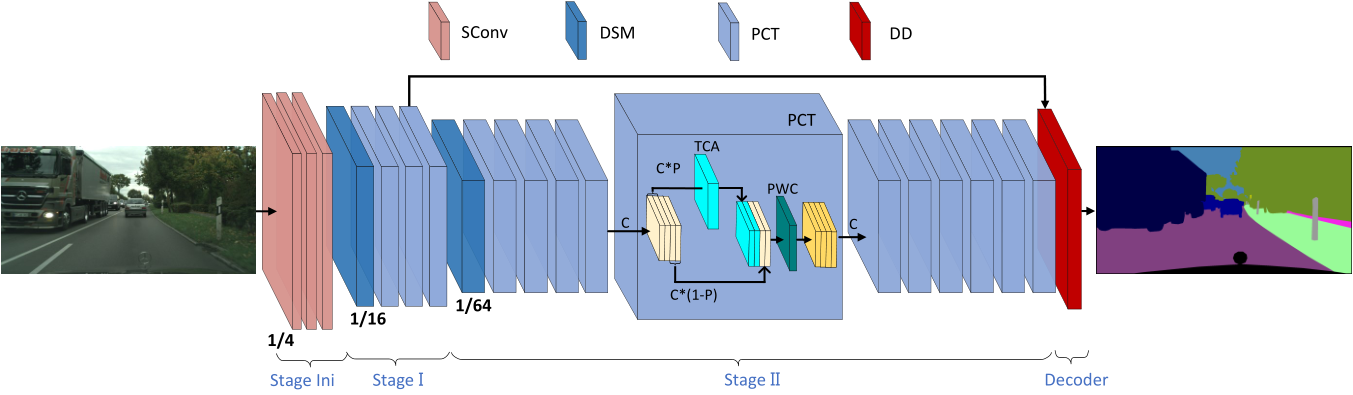
\includegraphics[width=\textwidth]{Images/LCNet.png}
    \caption{Overview of the LCNet architecture.
    Original diagram provided by the authors of \cite{shi2024lcnet}.}
    \label{fig:lcnet-architecture}
\end{figure}

Its main processing unit is the Partial-Channel Transformation (PCT) block, which splits the input features into two groups. One group passes directly to the output fusion, while the other undergoes context processing. The two groups are then concatenated and combined through a pointwise convolution \cite{shi2024lcnet}. In the project implementation, each path receives half of the channels, limiting the amount of spatial processing while retaining information from both groups. The transformed group is processed by a Three-Branch Context Aggregation (TCA) module, where a standard convolution first produces intermediate features, which are then processed by local and dilated depthwise convolutions. Their outputs are added to the intermediate features, combining information from nearby positions and wider regions without further downsampling.

\begin{figure}[htbp]
    \centering
    \begin{minipage}[c]{0.48\textwidth}
        \centering
        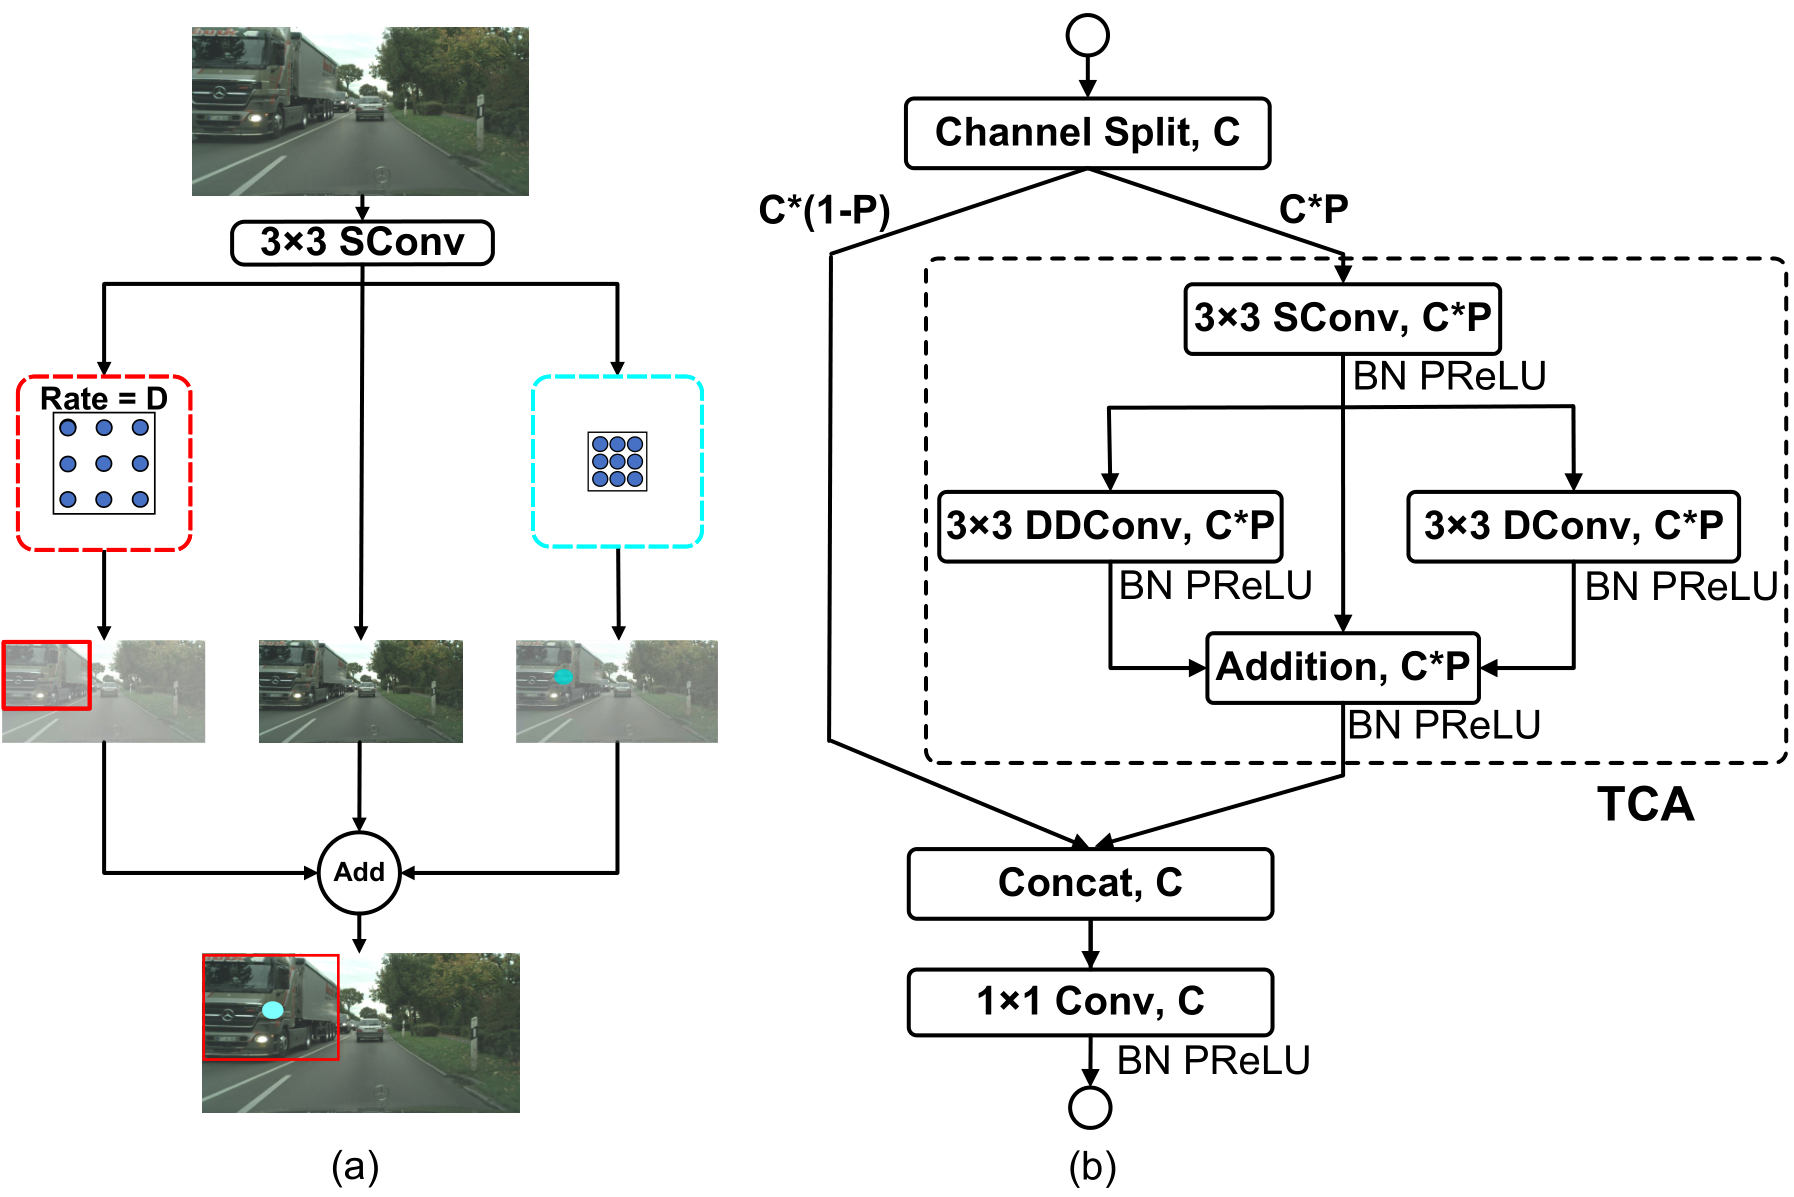
\includegraphics[width=\linewidth]{Images/lcnet_pct.png}
    \end{minipage}
    \hfill
    \begin{minipage}[c]{0.48\textwidth}
        \centering
        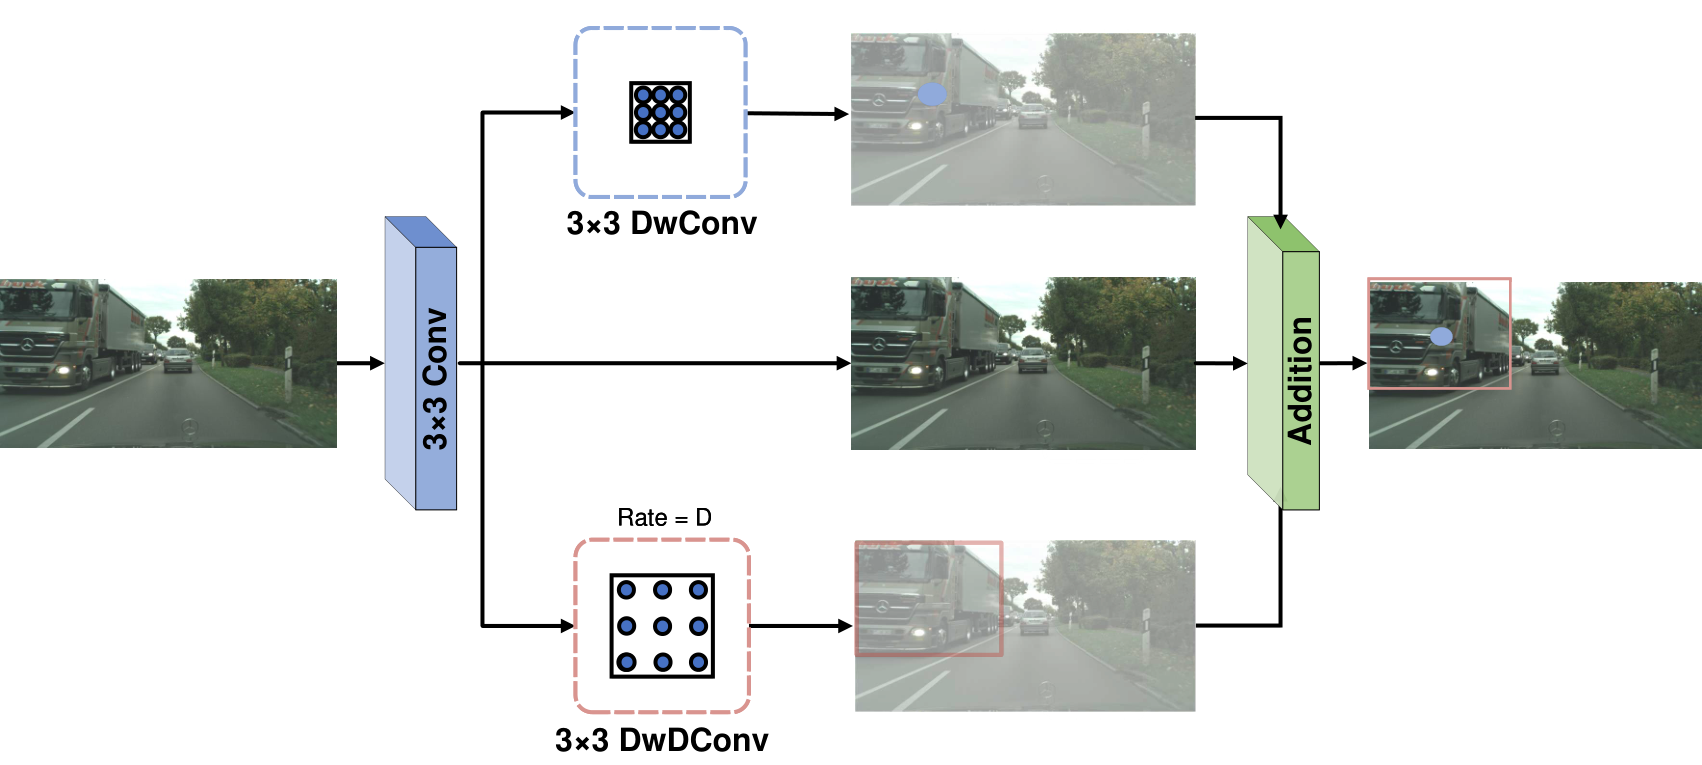
\includegraphics[width=\linewidth]{Images/lcnet_tca.png}
    \end{minipage}
    \caption{Partial-channel transformation (left) and three-branch
    context aggregation (right). Original diagrams provided by the
    authors of \cite{shi2024lcnet}.}
    \label{fig:lcnet-pct-tca}
\end{figure}

The encoder contains an initial convolutional stage followed by two PCT blocks. Each PCT stage begins with a downsampling block that combines a strided convolution with max pooling, so most context processing takes place at reduced spatial resolutions. The decoder then brings together features from both stages through two attention mechanisms \cite{shi2024lcnet}. The shallower features provide spatial guidance, while the deeper features are refined through a reverse-guidance branch. After resizing the deeper features, the decoder combines them with the spatial guidance through element-wise multiplication. A depthwise convolution and a pointwise classifier produce the class scores, which are resized to the input resolution using bilinear interpolation.

Two configurations were implemented: LCNet$_{3,7}$ and LCNet$_{3,11}$. Both use three PCT blocks in the first encoder stage, followed by seven and eleven blocks in the second stage, respectively. LCNet$_{3,11}$ therefore adds four context-processing blocks without changing the overall design, allowing the comparison to examine whether a deeper encoder offers enough additional accuracy to justify its computational cost. Both variants were independently reimplemented for the project and configured to predict the nine S5Mars classes. They use random initialization rather than pretrained weights, unlike the other model families. This difference must be considered when interpreting the comparison, since the models differ not only in architecture but also in their starting weights.

\subsection{Architectural Comparison}

Table~\ref{tab:segmentation-architecture-static-comparison} compares the seven configurations independently of their predictive performance. Parameter counts refer to the nine-class implementations used for S5Mars and include all trainable layers. The reported FP32 storage is the theoretical memory required by the parameters alone and excludes intermediate activations, framework metadata, buffers, and optimizer state.

\begin{table}[ht!]
    \centering
    \small
    \resizebox{\linewidth}{!}{%
    \begin{tabular}{@{}l l l r r@{}}
        \toprule
        \textbf{Model} &
        \textbf{Encoder} &
        \textbf{Initialization} &
        \textbf{Params. (M)} &
        \textbf{FP32 (MiB)} \\
        \midrule
        \midrule
        U-Net
        & ResNet-34
        & ImageNet
        & 24.438 & 93.22 \\

        U-Net
        & MobileNetV2
        & ImageNet
        & 6.630 & 25.29 \\

        DeepLabV3
        & ResNet-34
        \linebreak
        & ImageNet
        & 26.009 & 99.22 \\

        DeepLabV3+
        & MobileNetV2
        & ImageNet
        & 4.381 & 16.71 \\

        SegFormer-B0
        & MiT-B0
        & ADE20K
        & 3.716 & 14.18 \\

        LCNet$_{3,7}$
        & LCNet stem
        & Random
        & 0.509 & 1.94 \\

        LCNet$_{3,11}$
        & LCNet stem
        & Random
        & 0.729 & 2.78 \\
        \bottomrule
    \end{tabular}
    }
    \vspace{5mm}
    \caption{Comparison of the segmentation architectures implemented for the nine-class S5Mars task. Parameter storage is calculated as four bytes per parameter and reported in Megabytes.}
    \label{tab:segmentation-architecture-static-comparison}
\end{table}

\section{Training}

The segmentation models share a configurable training pipeline that controls the optimization procedure, loss function, data sampling, and checkpoint selection. A common reference configuration provides a consistent training budget across the architecture families, while allowing individual components to be modified for the ablation studies. Each architecture was trained for a maximum of 30 epochs with a batch size of 32, with images processed at the ($512 \times 512$) resolution defined in the preprocessing section. The pretrained models are fine-tuned end to end, therefore all network parameters remain trainable throughout optimization, including the encoders initialized from pretrained weights, whereas the LCNet configurations are optimized from random initialization. The training images are shuffled at every epoch, while validation and test samples are processed without shuffling or stochastic augmentation.

The loss function combines pixel-wise cross-entropy with Generalized Dice Loss:
\begin{equation}
\mathcal{L}
=
\alpha \mathcal{L}{\mathrm{CE}}
+
(1-\alpha)\mathcal{L}{\mathrm{GDL}},
\qquad \alpha = 0.5.
\label{eq}
\end{equation}
Cross-entropy supervises the probability assigned to the target class at each pixel, whereas the Dice component measures agreement between the predicted probability maps and the target regions. Generalized Dice introduces class-dependent weighting to account for differences in region size, following the formulation investigated by Sudre et al. for imbalanced segmentation tasks \cite{sudre2017generalizeddice}. Combining the two terms therefore provides pixel-wise classification supervision alongside a region-overlap objective. This follows the rationale to combine the gradient stability of cross-entropy with the ability of Dice-based losses to handle class imbalance \cite{yeung2022unified}.

In the implemented Generalized Dice loss, class volumes are computed from the target masks across the current mini-batch. Classes present in the batch receive weights inversely proportional to the square of their pixel counts, while absent classes receive zero weight in the Dice calculation. These weights are recomputed for each batch rather than derived from precomputed class frequency scores. A smoothing constant of $(10^{-5})$ is added to the numerator and denominator of the overlap ratio. The pipeline also supports a single loss function alone and alternative Dice weighting schemes. The available configurations include inverse-volume weighting or uniform weights over the classes present in the batch. These alternatives allow the contribution of the loss formulation to be examined separately from changes in architecture.

The Optimizer is AdamW \cite{loshchilov2019adamw}, with a base learning rate of \(10^{-4}\) and a weight-decay coefficient of \(10^{-2}\). A linear warm-up during the first epoch is followed by cosine decay towards zero over the remaining epochs, without warm restarts \cite{loshchilov2017sgdr}. Training runs for the fixed epoch budget without early stopping, while the checkpoint with the best validation performance is retained for evaluation. Training was performed on Kaggle using two NVIDIA T4 GPUs, each with 16 GB of VRAM.

\paragraph{Training-data sampling and optional augmentation.}

Standard sampling is the default configuration, while image oversampling is available as a separate training-only option. Unlike the class weighting inside Generalized Dice, which depends on pixel counts within a batch, oversampling uses the class frequency of the training images. It therefore modifies how frequently images are presented to the model without changing their masks or the loss definition. When oversampling is enabled, the number of training images containing each class is first computed. Each image receives the largest rarity factor among its eligible classes, where the rarity factor is the square root of the ratio between the most frequent class count and the count of the class under consideration. The image weights are capped at 5 before normalization, and images are sampled with replacement. With the reference epoch-length multiplier of 1, the number of samples equals the number of training images, preserving the nominal training length although some images may be repeated and others omitted in an epoch. 
Geometric augmentation is controlled independently from sampling and remains disabled in the default configuration. When enabled, the transformations described in the preprocessing section are applied jointly to each training image and its mask. Neither augmentation nor oversampling modifies the validation or test distributions.

\begin{table}[ht!]
\centering
\begin{tabular}{@{}l c@{}}
\toprule
\textbf{Setting} & \textbf{Default configuration} \\
\midrule
\midrule
Input resolution & $512 \times 512$ \\
Training epochs & 30 \\
Batch size & 32 \\
Trainable parameters & Entire network \\
Optimizer & AdamW \\
Base learning rate & \(10^{-4}\) \\
Weight decay & \(10^{-2}\) \\
Learning-rate schedule & Linear warm-up and cosine decay \\
Warm-up duration & 1 epoch \\
Loss Function & Cross-entropy and Generalized Dice \\
Cross-entropy coefficient \(\alpha\) & 0.5 \\
Dice class weighting & Inverse-square batch volume \\
Image-level oversampling & Disabled \\
Training augmentation & Disabled \\
Checkpoint selection & Highest validation mIoU \\
Random seed & 42 \\
\bottomrule
\end{tabular}
\vspace{5mm}
\caption{Reference configuration for semantic-segmentation training.
Experiment-specific changes to the loss, sampling, or augmentation
settings are reported with the corresponding evaluations.}
\label{tab}
\end{table}

\section{Evaluation Metrics}
\label{sec:segmentation-evaluation-metrics}

Segmentation performance is evaluated using pixel accuracy, per-class Intersection over Union (IoU), and mean Intersection over Union (mIoU), following established semantic-segmentation evaluation practice \cite{long2015fcn}. Predictions are obtained by selecting the highest-scoring class at each pixel, and the metrics are computed from a confusion matrix accumulated over the entire evaluated partition rather than averaged across images or mini-batches.

Let \(TP_c\), \(FP_c\), and \(FN_c\) denote the true-positive, false-positive, and false-negative pixel counts for class \(c\). The metrics are defined as
\begin{equation}
\begin{aligned}
    \mathrm{Pixel\ Accuracy}
    &= \frac{\sum_c TP_c}{N}, \\
    \mathrm{IoU}_c
    &= \frac{TP_c}{TP_c + FP_c + FN_c}, \\
    \mathrm{mIoU}
    &= \frac{1}{|\mathcal{C}_{+}|}
       \sum_{c \in \mathcal{C}_{+}} \mathrm{IoU}_c,
\end{aligned}
\label{eq:segmentation-evaluation-metrics}
\end{equation}
where \(N\) is the total number of evaluated pixels and \(\mathcal{C}_{+}\) contains the classes present in the ground truth of the evaluated partition.

Pixel accuracy measures the overall proportion of correctly classified pixels, but consequently gives greater influence to classes occupying larger image regions. In contrast, mIoU assigns equal weight to each included class and serves as the primary checkpoint-selection metric. Per-class IoU complements this aggregate measure by exposing differences between semantic categories that a single score may conceal.

% Computational efficiency is assessed separately through parameter count, estimated FLOPs, inference latency, and frames per second (FPS), with the hardware and measurement conditions specified in the evaluation chapter.

\section{Optimization and Quantization}
\label{sec:optimization-quantization}

Quantization was investigated to test the efficiency of the segmentation models for resource-constrained deployment, with the objective of reducing model storage and inference costs while preserving segmentation accuracy. Selected FP32 checkpoints were exported to ONNX as reference models, alongside FP16 variants obtained by converting eligible parameters and operations to half precision while maintaining FP32 inputs and outputs.

Static INT8 Post-Training Quantization (PTQ) was applied without retraining the models. Activation ranges were calibrated using 500 images sampled from the training set, without using their segmentation annotations. Selected weights and activations were quantized to signed, symmetric 8-bit integers, using per-channel quantization for weights and per-tensor quantization for activations. The quantized models used the ONNX Quantize/Dequantize (QDQ) format, which introduces explicit nodes to represent conversions between floating-point values and their quantized representations \cite{onnxruntimeQuantization}.

An alternative INT8 strategy was done with Quantization-Aware Training (QAT) using NVIDIA ModelOpt. Fake-quantization operations simulated rounding and clipping during fine-tuning, allowing the models to adapt to quantization effects \cite{jacob2018quantization}. The training objective combined the supervised segmentation loss with knowledge distillation from a frozen FP32 teacher. The resulting models were exported to ONNX with explicit quantization and dequantization operations, without an additional PTQ step.

Both INT8 strategies used selective quantization, keeping floating-point computations where required for compatibility or accuracy. For example, in the evaluated Conv-only configuration of SegFormer-B0, INT8 was restricted to convolutional layers, whereas linear projections, attention matrix multiplications, normalization, and softmax remained in floating point, with FP16 fallback in TensorRT. The resulting models therefore used mixed precision rather than an entirely integer computation graph. FP32, FP16, and PTQ inference relied on ONNX Runtime, whereas QAT models were executed directly with TensorRT. Quantization configurations were selected using the validation set, reserving the test set for final evaluation.